\documentclass[12pt, titlepage]{article}

\usepackage{fullpage}
\usepackage[round]{natbib}
\usepackage{multirow}
\usepackage{booktabs}
\usepackage{tabularx}
\usepackage{graphicx}
\usepackage{float}
\usepackage{hyperref}
\hypersetup{
    colorlinks,
    citecolor=blue,
    filecolor=black,
    linkcolor=red,
    urlcolor=blue
}

%% Comments

\usepackage{color}

\newif\ifcomments\commentstrue %displays comments
%\newif\ifcomments\commentsfalse %so that comments do not display

\ifcomments
\newcommand{\authornote}[3]{\textcolor{#1}{[#3 ---#2]}}
\newcommand{\todo}[1]{\textcolor{red}{[TODO: #1]}}
\else
\newcommand{\authornote}[3]{}
\newcommand{\todo}[1]{}
\fi

\newcommand{\wss}[1]{\authornote{blue}{SS}{#1}} 
\newcommand{\plt}[1]{\authornote{magenta}{TPLT}{#1}} %For explanation of the template
\newcommand{\an}[1]{\authornote{cyan}{Author}{#1}}

%% Common Parts

\newcommand{\progname}{ProgName} % PUT YOUR PROGRAM NAME HERE
\newcommand{\authname}{Team \#, Team Name
\\ Student 1 name
\\ Student 2 name
\\ Student 3 name
\\ Student 4 name} % AUTHOR NAMES                  

\usepackage{hyperref}
    \hypersetup{colorlinks=true, linkcolor=blue, citecolor=blue, filecolor=blue,
                urlcolor=blue, unicode=false}
    \urlstyle{same}
                                


\newcounter{acnum}
\newcommand{\actheacnum}{AC\theacnum}
\newcommand{\acref}[1]{AC\ref{#1}}

\newcounter{ucnum}
\newcommand{\uctheucnum}{UC\theucnum}
\newcommand{\uref}[1]{UC\ref{#1}}

\newcounter{mnum}
\newcommand{\mthemnum}{M\themnum}
\newcommand{\mref}[1]{M\ref{#1}}

\begin{document}

\title{Module Guide for \progname{}} 
\author{\authname}
\date{\today}

\maketitle

\pagenumbering{roman}

\section{Revision History}

\begin{tabularx}{\textwidth}{p{3cm}p{2cm}X}
\toprule {\bf Date} & {\bf Developer} & {\bf Notes/Changes}\\
\midrule
Jan 15, 2023 & Timothy Chen & Added Anticipated and Unlikey Cahnges (4)\\
Jan 15, 2023 & Timothy & Added Module Hierarchy (5)\\
Jan 16, 2023 & Edwin Do & Add use hierarchy diagram \\
Jan 18, 2023 & Edwin Do & Add traceability matrices \\
Jan 18, 2023 & Tyler Magarelli & Added Module Decomposition \\

\bottomrule
\end{tabularx}

\newpage

\section{Reference Material}

This section records information for easy reference.

\subsection{Abbreviations and Acronyms}

\renewcommand{\arraystretch}{1.2}
\begin{tabular}{l l} 
  \toprule		
  \textbf{symbol} & \textbf{description}\\
  \midrule 
  AC & Anticipated Change\\
  DAG & Directed Acyclic Graph \\
  M & Module \\
  MG & Module Guide \\
  OS & Operating System \\
  R & Requirement\\
  SC & Scientific Computing \\
  SRS & Software Requirements Specification\\
  \progname & Explanation of program name\\
  UC & Unlikely Change \\
  \bottomrule
\end{tabular}\\

\newpage

\tableofcontents

\listoftables

\listoffigures

\newpage

\pagenumbering{arabic}

\section{Introduction}

Decomposing a system into modules is a commonly accepted approach to developing
software.  A module is a work assignment for a programmer or programming
team~\citep{ParnasEtAl1984}.  We advocate a decomposition
based on the principle of information hiding~\citep{Parnas1972a}.  This
principle supports design for change, because the ``secrets'' that each module
hides represent likely future changes.  Design for change is valuable in SC,
where modifications are frequent, especially during initial development as the
solution space is explored.  

Our design follows the rules layed out by \citet{ParnasEtAl1984}, as follows:
\begin{itemize}
\item System details that are likely to change independently should be the
  secrets of separate modules.
\item Each data structure is implemented in only one module.
\item Any other program that requires information stored in a module's data
  structures must obtain it by calling access programs belonging to that module.
\end{itemize}

After completing the first stage of the design, the Software Requirements
Specification (SRS), the Module Guide (MG) is developed~\citep{ParnasEtAl1984}. The MG
specifies the modular structure of the system and is intended to allow both
designers and maintainers to easily identify the parts of the software.  The
potential readers of this document are as follows:

\begin{itemize}
\item New project members: This document can be a guide for a new project member
  to easily understand the overall structure and quickly find the
  relevant modules they are searching for.
\item Maintainers: The hierarchical structure of the module guide improves the
  maintainers' understanding when they need to make changes to the system. It is
  important for a maintainer to update the relevant sections of the document
  after changes have been made.
\item Designers: Once the module guide has been written, it can be used to
  check for consistency, feasibility, and flexibility. Designers can verify the
  system in various ways, such as consistency among modules, feasibility of the
  decomposition, and flexibility of the design.
\end{itemize}

The rest of the document is organized as follows. Section
\ref{SecChange} lists the anticipated and unlikely changes of the software
requirements. Section \ref{SecMH} summarizes the module decomposition that
was constructed according to the likely changes. Section \ref{SecConnection}
specifies the connections between the software requirements and the
modules. Section \ref{SecMD} gives a detailed description of the
modules. Section \ref{SecTM} includes two traceability matrices. One checks
the completeness of the design against the requirements provided in the SRS. The
other shows the relation between anticipated changes and the modules. Section
\ref{SecUse} describes the use relation between modules.

\section{Anticipated and Unlikely Changes} \label{SecChange}

This section lists possible changes to the system. According to the likeliness
of the change, the possible changes are classified into two
categories. Anticipated changes are listed in Section \ref{SecAchange}, and
unlikely changes are listed in Section \ref{SecUchange}.

\subsection{Anticipated Changes} \label{SecAchange}

Anticipated changes are the source of the information that is to be hidden
inside the modules. Ideally, changing one of the anticipated changes will only
require changing the one module that hides the associated decision. The approach
adapted here is called design for
change.

\begin{description}
\item[\refstepcounter{acnum} \actheacnum \label{acHardware}:] The specific
  hardware on which the software is running.
\item[\refstepcounter{acnum} \actheacnum \label{acInput}:] The format of the
  input data from the user.
\item[\refstepcounter{acnum} \actheacnum \label{acOutput}:] The format of the output data.
\item[\refstepcounter{acnum} \actheacnum \label{acCalculation}:] The number of calculations the application will peform.
\item[\refstepcounter{acnum} \actheacnum \label{acGraph}:] The number and type of graphs displayed.
\item[\refstepcounter{acnum} \actheacnum \label{acNumInput}:] The number of inputs the user can provide.
\item[\refstepcounter{acnum} \actheacnum \label{acValidation}:] The criteria for validing data within the application.
\end{description}

\subsection{Unlikely Changes} \label{SecUchange}

The module design should be as general as possible. However, a general system is
more complex. Sometimes this complexity is not necessary. Fixing some design
decisions at the system architecture stage can simplify the software design. If
these decision should later need to be changed, then many parts of the design
will potentially need to be modified. Hence, it is not intended that these
decisions will be changed.

\begin{description}
\item[\refstepcounter{ucnum} \uctheucnum \label{ucIO}:] Input/Output devices
  (Input: File and/or Keyboard, Output: File, Memory, and/or Screen, Measurement Equipment).
\item[\refstepcounter{ucnum} \uctheucnum \label{ucOS}:] Operating system (Windows 10).
\item[\refstepcounter{ucnum} \uctheucnum \label{ucCalculation}:] Calculation equation formulas (Resistance equation and Resistivity equation).
\end{description}

\section{Module Hierarchy} \label{SecMH}

This section provides an overview of the module design. Modules are summarized
in a hierarchy decomposed by secrets in Table \ref{TblMH}. The modules listed
below, which are leaves in the hierarchy tree, are the modules that will
actually be implemented.

\begin{description}
\item [\refstepcounter{mnum} \mthemnum \label{mHH}:] Hardware-Hiding Module
\item [\refstepcounter{mnum} \mthemnum \label{mIC}:] Input Communication Module
\item [\refstepcounter{mnum} \mthemnum \label{mOC}:] Output Communication Module
\item [\refstepcounter{mnum} \mthemnum \label{mRA}:] Remote Access Module
\item [\refstepcounter{mnum} \mthemnum \label{mCS}:] Current State Module
\item [\refstepcounter{mnum} \mthemnum \label{mFO}:] File Output Module
\item [\refstepcounter{mnum} \mthemnum \label{mGO}:] Graphical Output Module
\item [\refstepcounter{mnum} \mthemnum \label{mC}:] Calculation Module
\item [\refstepcounter{mnum} \mthemnum \label{mUI}:] User Input Validation Module
\item [\refstepcounter{mnum} \mthemnum \label{mHI}:] Hardware Input Validation Module
\end{description}


\begin{table}[h!]
\centering
\begin{tabular}{p{0.3\textwidth} p{0.6\textwidth}}
\toprule
\textbf{Level 1} & \textbf{Level 2}\\
\midrule

{Hardware-Hiding Module} & ~ \\
\midrule

\multirow{7}{0.3\textwidth}{Behaviour-Hiding Module}
& Input Cummication Module\\
& Output Communication Module\\
& Remote Access Module\\
& Current State Module\\
& FileOutput Module\\
& Graphical Output Module\\ 
\midrule

\multirow{3}{0.3\textwidth}{Software Decision Module}
& Calculation Module\\
& User Input Validation Module \\
& Hardware Input Validation Module\\ 
\bottomrule

\end{tabular}
\caption{Module Hierarchy}
\label{TblMH}
\end{table}

\section{Connection Between Requirements and Design} \label{SecConnection}

The design of the system is intended to satisfy the requirements developed in
the SRS. In this stage, the system is decomposed into modules. The connection
between requirements and modules is listed in Table~\ref{TblRT}.

\section{Module Decomposition} \label{SecMD}

\subsection{Hardware Hiding Modules (\mref{mHH})}

\begin{description}
\item[Secrets:]The data structure and algorithm used to implement the hardware.
\item[Services:]This module provides the interface between the hardware and the
  software. So, the system can use it to display outputs or to accept inputs.
\item[Implemented By:] OS
\end{description}

\subsection{Behaviour-Hiding Module}

\subsubsection{Communication Module}
\begin{description}
  \item[Secrets:] Format input and output data and manage remote connection communication.
  \item[Services:]Converts the data into the appropriate data structure used by the
    input/output parameters module. Controls communication for remote access. 
  \item[Implemented By:] -
  \end{description}

\paragraph{Input Communication Module (\mref{mIC})}
\begin{description}
\item[Secrets:]The format and structure of the input data (temperature, etc.)
\item[Services:]Converts the input data into the data structure used by the
  input parameters module.
\item[Implemented By:] Communication.cs
\item[Type of Module:] Abstract Data Type
\end{description}

\paragraph{Output Communication Module (\mref{mOC})}
\begin{description}
\item[Secrets:]The format and structure of the output data.
\item[Services:]Converts the output data into the data structure used by the output parameters module. 
\item[Implemented By:] Communication.cs
\item[Type of Module:] Abstract Data Type
\end{description}

\paragraph{Remote Access Module (\mref{mRA})}
\begin{description}
\item[Secrets:]The implementation and algorithm of remote access. Login info and other credentials required for remote connection.
\item[Services:]Remote acces to the application for the user.
\item[Implemented By:] RemoteAccess.cs
\item[Type of Module:] Abstract Object Type
\end{description}

\subsubsection{Display Module}
\begin{description}
  \item[Secrets:] Display output data and and other information to the user.
  \item[Services:]Receives data to be displayed and displays it on the screen for the user to see. 
  \item[Implemented By:] -
\end{description}

\paragraph{Current State Module (\mref{mCS})}
\begin{description}
\item[Secrets:]The contents of obtaining current system state.
\item[Services:]Display state of hardware (current temp, current voltage, current sampling rate, etc.)
\item[Implemented By:] CurrentState.cs
\item[Type of Module:] Abstract Data Type
\end{description}

\paragraph{File Output Module (\mref{mFO})}
\begin{description}
\item[Secrets:]The contents of obtaining correct files for output.
\item[Services:]Outputs the file the to screen for the user. 
\item[Implemented By:] FileOutput.cs
\item[Type of Module:] Record
\end{description}
\paragraph{Graphical Output Module (\mref{mGO})}
\begin{description}
\item[Secrets:]Obtaining the correct data to produce accurate graphs.
\item[Services:]Displays the data in a graphical format. 
\item[Implemented By:] Graph.cs
\item[Type of Module:] Abstract Object Type
\end{description}

\subsection{Software Decision Module}

\paragraph{Calculation Module (\mref{mC})}
\begin{description}
  \item[Secrets:] The mathematical equation for calculating resistivity and resistance.
  \item[Services:]Solve the equation for resistivity and resistance respectively and return the result.
  \item[Implemented By:] Calculation.cs 
  \item[Type of Module:] Abstract Data Type
\end{description}

\subsubsection{Validation Module}
\begin{description}
  \item[Secrets:] Validation criteria for various input streams.
  \item[Services:]Validates the correctness of provided input from the given stream.
  \item[Implemented By:] -
\end{description}

\paragraph{User Input Validation Module (\mref{mUI})}
\begin{description}
  \item[Secrets:] Validation criteria for user input.
  \item[Services:] Validates the input from the user.
  \item[Implemented By:] UserValidation.cs 
  \item[Type of Module:] Abstract Data Type
\end{description}

\paragraph{Hardware Input Validation Module(\mref{mHI})}
\begin{description}
  \item[Secrets:] Validation criteria for hardware input.
  \item[Services:] Validates the input from the hardware.
  \item[Implemented By:] HardwareValidation.cs 
  \item[Type of Module:] Abstract Data Type
\end{description}

\section{Traceability Matrix} \label{SecTM}

This section shows two traceability matrices: between the modules and the
requirements and between the modules and the anticipated changes.

% the table should use mref, the requirements should be named, use something
% like fref
\begin{table}[H]
\centering
\begin{tabular}{p{0.2\textwidth} p{0.6\textwidth}}
\toprule
\textbf{Req.} & \textbf{Modules}\\
\midrule
R1 & \mref{mRA}, \mref{mCS}\\
R2 & \mref{mFO}, \mref{mGO}, \mref{mC}\\
R3 & \mref{mIC}\\
R4 & \mref{mFO}, \mref{mGO}, \mref{mC}\\
R5 & \mref{mRA}\\
\bottomrule
\end{tabular}
\caption{Trace Between Requirements and Modules}
\label{TblRT}
\end{table}

\begin{table}[H]
\centering
\begin{tabular}{p{0.2\textwidth} p{0.6\textwidth}}
\toprule
\textbf{AC} & \textbf{Modules}\\
\midrule
\acref{acHardware} & \mref{mHH}\\
\acref{acInput} & \mref{mIC}\\
\acref{acOutput} & \mref{mOC}\\
\acref{acCalculation} & \mref{mC}\\
\acref{acGraph} & \mref{mGO}\\
\acref{acNumInput} & \mref{mIC}\\
\acref{acValidation} & \mref{mUI}\\
\bottomrule
\end{tabular}
\caption{Trace Between Anticipated Changes and Modules}
\label{TblACT}
\end{table}

\section{Use Hierarchy Between Modules} \label{SecUse}

In this section, the uses hierarchy between modules is
provided. \citet{Parnas1978} said of two programs A and B that A {\em uses} B if
correct execution of B may be necessary for A to complete the task described in
its specification. That is, A {\em uses} B if there exist situations in which
the correct functioning of A depends upon the availability of a correct
implementation of B.  Figure \ref{FigUH} illustrates the use relation between
the modules. It can be seen that the graph is a directed acyclic graph
(DAG). Each level of the hierarchy offers a testable and usable subset of the
system, and modules in the higher level of the hierarchy are essentially simpler
because they use modules from the lower levels.


\begin{figure}[H]
\centering
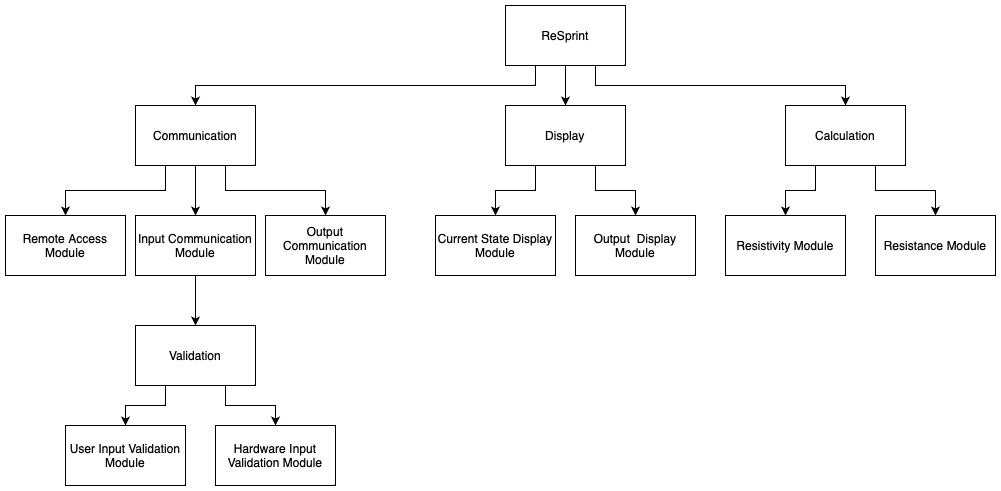
\includegraphics[width=0.7\textwidth]{UsesHierarchy.png}
\caption{Use hierarchy among modules}
\label{FigUH}
\end{figure}

%\section*{References}

\bibliographystyle {plainnat}
\bibliography{../../../refs/References}

\newpage{}

\end{document}